\documentclass{beamer}

\usepackage{graphicx} % Required for inserting images
\usepackage[slovene]{babel}



\mode<presentation>

\usetheme{Berkeley}
\usecolortheme{seahorse}

\logo{
\includegraphics[height=1cm]{fs-logo.jpg}}

\title{Domača Naloga 1}
\author{JAKA HATLAK}
\date{October 2023}

\begin{document}




\begin{frame}{\small Napredna Računalniška Ordoja}
    \titlepage
\end{frame}

\begin{frame}{\small Kazalo}
    \tableofcontents
\end{frame}

\section{Uvod}
\begin{frame}{\small Uvod}
    Pri prvi domači nalogi smo se učili uporabljati:
    \begin{itemize}
        \item{MATLAB}
        \pause
        \item{GitHub}
        \pause
        \item{LaTeX}
    \end{itemize}
    
\end{frame}

\begin{frame}{\small Kazalo}
    \tableofcontents
\end{frame}

\section{MATLAB}
\begin{frame}{\small MATLAB}
    V matlabu smo s pomočjo monte carlo metode iskali približek števila $\pi$, koraki za izračun števila $pi$ so:
        \begin{itemize}
        \item{Znotraj kvadrata generiramo veliko število naključnih točk}
        \pause
        \item{Preverimo ali so točke znotraj kvadratu včrtanega kroga}
        \pause
        \item{Izračunamo razmerje  števila točk znotraj kroga proti številu točk zunaj kroga $$\frac{\textnormal{št. točk v krogu}}{\textnormal{št. vseh točk}}$$}
    \end{itemize}
    
\end{frame}

\begin{frame}{\small MATLAB}
    Te točke lahko na četrtini kroga tudi izrišemo:
    \begin{figure}
        \centering
        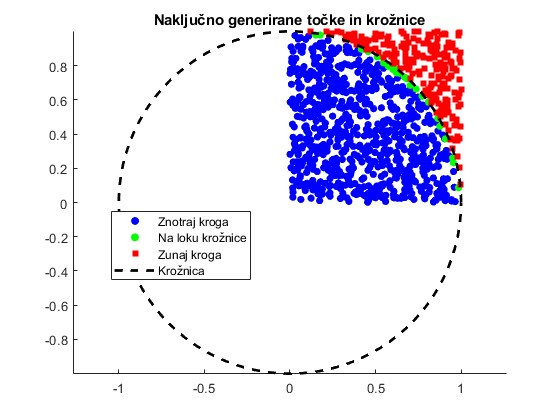
\includegraphics[scale=0.38]{točke.jpg}
        \caption{Točke izrisane za četrtino kroga}
        \label{KROG}
    \end{figure}
\end{frame}

\begin{frame}{\small Kazalo}
    \tableofcontents
\end{frame}

\section{GitHub}
\begin{frame}{\small GitHub}
    S pomočji GitHuba smo se naučili enostavne kolaboracije na projektih z več udeleženci, kjer lahko vsak udeleženec poljubno spreminja kodo, s pomočjo funkcije 'pull request'.

    \begin{figure}
        \centering
        
\includegraphics[scale=0.05]{GitHub-logo.png}
        \caption{GitHub logo}
        \label{GITHUB}
    \end{figure}
\end{frame}

\begin{frame}{\small Kazalo}
    \tableofcontents
\end{frame}

\section{LaTeX}
\begin{frame}{\small LaTeX}
    LaTeX, pa nam omogoča enostavno in predvsem hitro kreiranje člankov, predstavitev, knjig in še mnogo drugega, saj v njem definiramo ves izgled že na začetku in se kasneje ne ukvarjamo z njim. Na ta način se lahko fokusiramo na vsebino. 
    
    \vspace{0.5cm}
    \pause
    Glavne kvalitete LaTeX-a so:
    \begin{itemize}
        \item{Hitrost}
        \pause
        \item{Enostavnost (predvsem v matematičnih izrazih)}
        \pause
        \item{Ponovljivost izdelave}
    \end{itemize}
    
\end{frame}

\end{document}